\documentclass[conference]{IEEEtran}
\usepackage{amsmath}
\DeclareMathOperator\arctanh{arctanh}
\usepackage{amsfonts}
\usepackage{gensymb}
\usepackage{graphicx}
\usepackage{url}
\usepackage{amsmath}
\usepackage{color}
\usepackage{xfrac}
\usepackage{flushend}
\usepackage{wrapfig}
\usepackage{float}
\usepackage{csvsimple}
\usepackage{textgreek}
\usepackage{siunitx}

\newcommand*{\Scale}[2][4]{\scalebox{#1}{$#2$}}%

\makeatletter \renewcommand*\env@matrix[1][*\c@MaxMatrixCols c]{ \hskip
    -\arraycolsep \let\@ifnextchar\new@ifnextchar \array{#1}} \makeatother

\graphicspath{{./img/}}

\begin{document}

\title{Lab 5: Transmission Line Measurements}
\author{
    \IEEEauthorblockN{John McAvoy, James Merrill}
    \IEEEauthorblockA{
        ECE 09.303, Section 4\\
        17 December 2018\\
        Emails: (mcavoyj5,merrillj1)@students.rowan.edu
    }
}
\maketitle
\IEEEpeerreviewmaketitle

\begin{abstract}
%TODO Reword abstract
In this lab, the transmission line properties, such as $\gamma$, $Z_0$, $Z_L$
and $Z_{in}$; of a coaxial cable were measured. The effect of six different
load impedances: \SI{47}{\ohm}, \SI{50}{\ohm},\SI{100}{\ohm},
\SI{2.2}{\pico\farad}, $0$, and $\infty$, on these values was measured using a
network analyzer. Using fundamental transmission line equations, the
theoretical $V_0^-$ reflection of a generated pulse was accurately predicted.
Additionally theoretical values for $Z_0$ and $\gamma$ for the transmission line
were determined used to compare the expected load impedances from the network
analyzer's data to the actual loads.

\end{abstract}

\section{Introduction and Objectives}
%TODO
The purpose of this lab is to explore the properties of transmission lines and
observe the effect that a load has on signal reflections. This lab is broken
into three parts:

\begin{enumerate}
  \item{Observing Wave Reflection}
    A single, short pulse was generated and sent down a \SI{30}{\meter} long coaxial cable
    and the voltage at the generator end of the cable was measured using an
    oscilloscope. The pulse's width and the cable's length were chosen such that
    the reflected wave would clearly appear at the generator end as a separate
    pulse a ~250 ns after the signal is sent. The reflected wave of the same
    transmission line with the following terminations were observed:

    \begin{table}[H]
      \renewcommand{\arraystretch}{1.3}
      \caption{Terminations}
      \label{terminations}
      \centering
      \begin{tabular}{c||c}
        \hline
        \bfseries Termination & \bfseries $Z_L$\\
        \hline\hline
        \SI{47}{\ohm} Resistor           & $47$                             \\
        \SI{50}{\ohm} Resistor           & $50$                             \\
        \SI{100}{\ohm} Resistor          & $100$                            \\
        \SI{2.2}{\nano\farad} Capacitor  & $\frac{1}{j\omega\num{2.2e-9} } $\\
        Short Circuit                    & $0$                              \\
        Open Circuit                     & $\infty$                         \\
        \hline
      \end{tabular}
    \end{table}

  \item{Measuring the Input Impedance}
    A network analyzer was used to measure the input impedance of the
    transmission line at 1.0 MHz, 10 MHz, 250 MHz, and 500 Mz for each of the
    six terminations.

  \item{Deriving Experimental $Z_L$ Values}
    Based on the measured values of $\gamma$ and $Z_0$, an experimental $Z_L$ is
    derived for all 6 terminations and at all four frequencies and compared to
    the known values.
\end{enumerate}

\section{Background and Relevant Theory}

\begin{enumerate}
  \item Voltage Seen at Generator
    \begin{equation}{\label{eq:voltage_seen_at_generator}}
      V(z) = V_0^+ e^{-\gamma z} + V_0^- e^{\gamma z}
    \end{equation}

  \item Complex Propagation Constant
    \begin{equation}{\label{eq:propagation_constant}}
      \gamma = \sqrt{(R + j \omega L) (G + j \omega C)}\\
    \end{equation}

  \item Complex Propagation Constant: Lossless Line
    \begin{equation}{\label{eq:propagation_constant_lossless}}
      \begin{array}{ll}
        R = G = 0\\
        \gamma = j \omega \sqrt{L C} = \alpha + j \beta\\
        \alpha = 0\\
        \gamma = j \beta = j \omega \sqrt{LC}
      \end{array}
    \end{equation}

  \item Reflection Coefficient
    \begin{equation}{\label{eq:reflection_coefficient}}
      \Gamma = \frac{V_0^-}{V_0^+}=\frac{Z_L-Z_0}{Z_L+Z_0}
    \end{equation}

  \item Input Impedance
    \begin{equation}{\label{eq:z_in}}
      Z_{in} = Z_0 \frac{Z_L + Z_0 \tanh{\gamma l}}{Z_0 + Z_L \tanh{\gamma l}}
    \end{equation}

  \item Characteristic Impedance
    \begin{equation}{\label{eq:z_0}}
      Z_0 = \sqrt{Z_i^{OC} Z_i^{SC}}
    \end{equation}

\end{enumerate}

\section{Results and Discussion}

\subsection{Observing Wave Reflection}

\subsubsection{\SI{47}{\ohm} Resistor}

\begin{figure}[H]
  \centering
  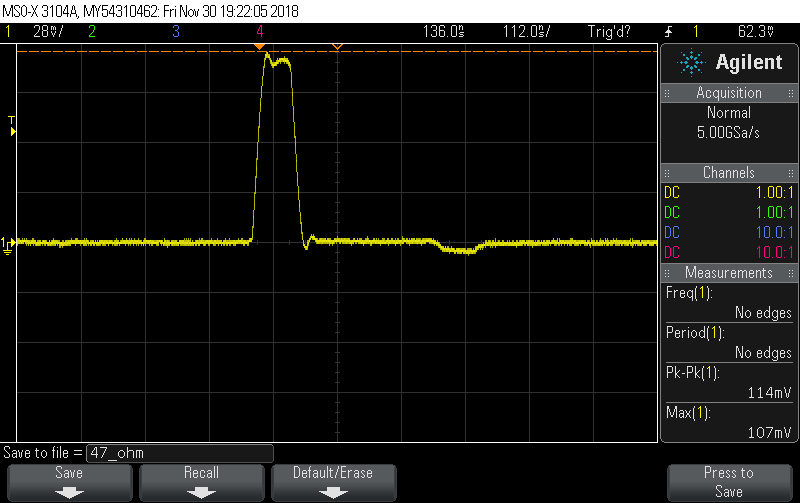
\includegraphics[width=2.5in]{./img/47_ohm.png}
  \caption{Voltage Seen at Generator: \SI{47}{\ohm} Resistor}
  \label{fig:47_ohm}
\end{figure}

The reflected voltage wave is expected to be an inversion of the input, in the
case of a \SI{100}{\milli\volt} pulse, the reflected signal should be
a \SI{-3.1}{\milli\volt} pulse (Equation \ref{eq:v_reflected_47_ohms}). The
theoretical value accurately predicted the observed reflected wave, the observed
reflection voltage was a \SI{-5}{\milli\volt} signal (Figure \ref{fig:47_ohm}).


\subsubsection{\SI{50}{\ohm} Resistor}
\begin{figure}[H]
  \centering
  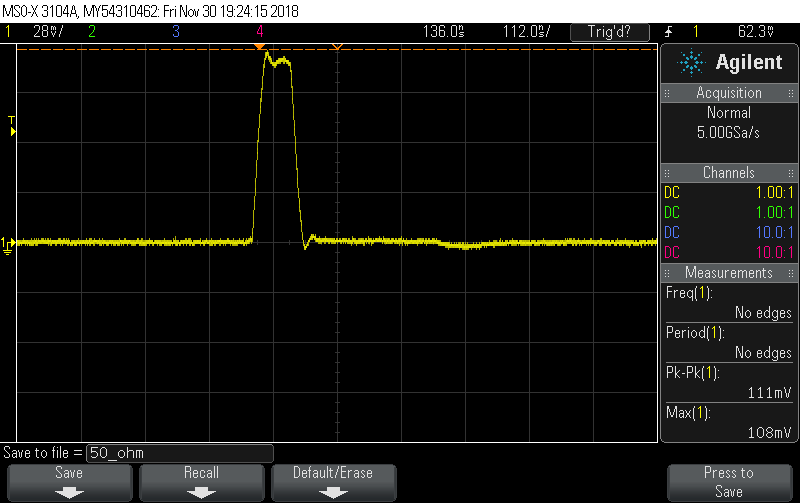
\includegraphics[width=2.5in]{./img/50_ohm.png}
  \caption{Voltage Seen at Generator: \SI{50}{\ohm} Resistor}
  \label{fig:50_ohm}
\end{figure}

The reflected voltage wave for the \SI{50}{\ohm} load is expected to be zero regardless of the voltage
input (Equation \ref{eq:v_reflected_50_ohms}). This prediction was accurate,
there is almost no reflected wave (Figure \ref{fig:50_ohm}).

\subsubsection{\SI{100}{\ohm} Resistor}
\begin{figure}[H]
  \centering
  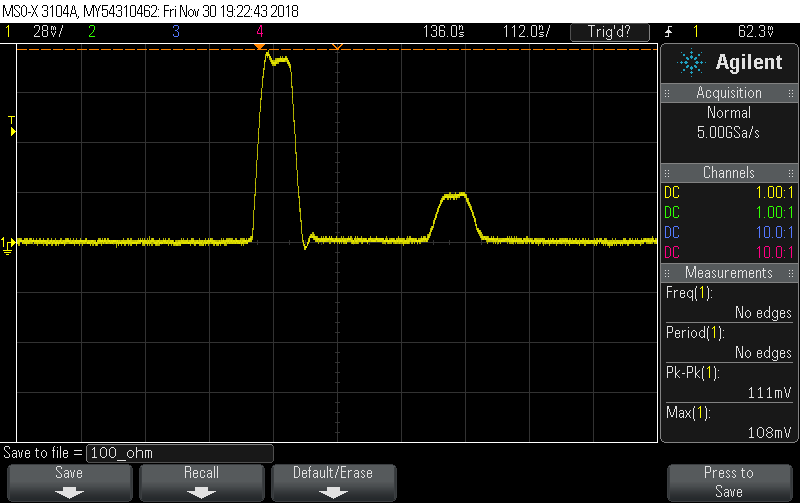
\includegraphics[width=2.5in]{./img/100_ohm.png}
  \caption{Voltage Seen at Generator: \SI{100}{\ohm} Resistor}
  \label{fig:100_ohm}
\end{figure}

The reflected voltage wave for the \SI{100}{\ohm} load is expected to be a third of the input
voltage (Equation \ref{eq:v_reflected_100_ohms}). In this case, the same square
pulse but with an amplitude of \SI{33.3}{\milli\volt}.

\subsubsection{\SI{2.2}{\pico\farad} Capacitor}
\begin{figure}[H]
  \centering
  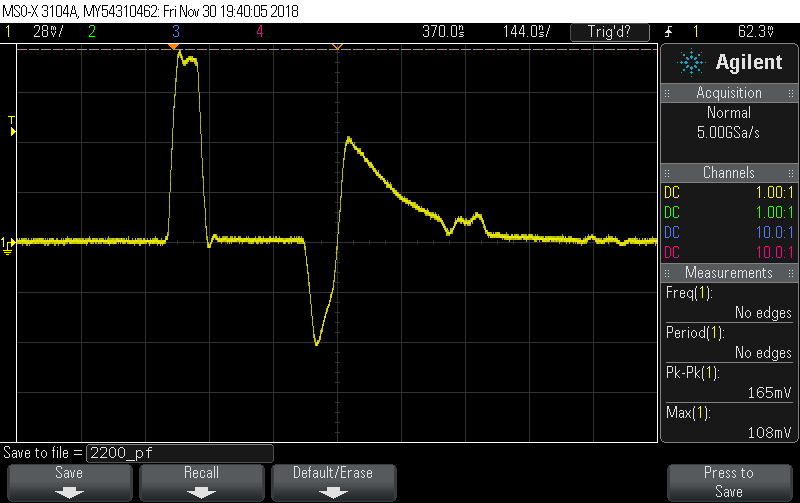
\includegraphics[width=2.5in]{./img/2200_pf.png}
  \caption{Voltage Seen at Generator: \SI{22.2}{\pico\farad} Capacitor}
  \label{fig:2200_pf}
\end{figure}

The reflected voltage wave for the \SI{2.2}{\pico\farad} load is expected to
have a complex $V_0^-$, meaning the reflected voltage will depend on the
frequency of the input voltage. Since a square pulse is used, the reflected wave
is not obvious since all frequencies are theoretically contained in the pulse.
The reflection observed fits this characteristic since it has a non-square shape
and it is has both an inverting and non-inverting peak (Figure
\ref{fig:2200_pf}).

\subsubsection{Short Circuit}
\begin{figure}[H]
  \centering
  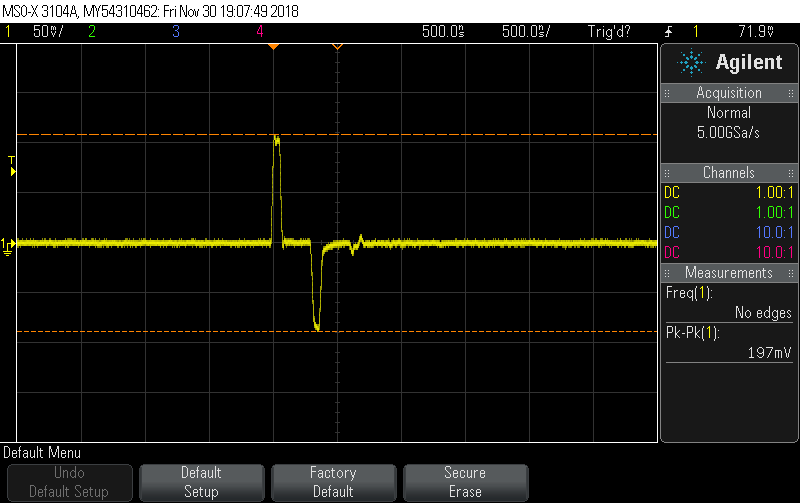
\includegraphics[width=2.5in]{./img/short.png}
  \caption{Voltage Seen at Generator: Short Circuit}
  \label{fig:short}
\end{figure}

The reflected voltage wave of the short circuit is expected to be an inversion of the input voltage,
a \SI{-100}{\milli\volt} pulse (Equation \ref{eq:v_reflected_short}). This was
observed as a \SI{-90}{\milli\volt} pulse (Figure \ref{fig:short}).

\subsubsection{Open Circuit}
\begin{figure}[H]
  \centering
  
\includegraphics[width=2.5in]{./img/open.png}
  \caption{Voltage Seen at Generator: Open Circuit}
  \label{fig:open}
\end{figure}

The reflected voltage wave of the open circuit is expected to be equal to the input voltage,
a \SI{100}{\milli\volt} pulse (Equation \ref{eq:v_reflected_open}). This was
observed as a \SI{90}{\milli\volt} pulse (Figure \ref{fig:open}).

\subsection{Measuring the Input Impedance}
The input impedance for all terminators were measured using a network analyzer
in $S_{11}$ configuration (Appendix B). The Smith chart readings of the input
impedances were used to derive experimental values for $Z_0$ and $\gamma$ by
using the input impedances for an open and short circuit (Appendix C). The
experimental values were determined to be $Z_0 = 62.12 + j3.30$ and $\gamma =
\num{4.86e-3} + j\num{2.713e-1}$ (Appendix C).

\subsection{Deriving Experimental $Z_L$ Values}
Using the derived $Z_0$ and $\gamma$ values, $Z_L$ for each load and at each
frequency was able to be determined (Appendix C). The theoretical load
impedances were not accurate at predicting the actual load impedances.

\section{Conclusion}

This lab was successful in observing the characteristics of a transmission line.
The predicted reflection waves for the generated pulse matched the observed
waveform, the intrinsic values of the transmission line were able to be
calculated accurately while the theoretical load impedances differed from the
actual values. This lab can be improved in the future by using a calibrated
network analyzer in order to get more accurate theoretical load impedances.

\begin{thebibliography}{99}

  \bibitem{ucdavis}
  F. Farahmand, "Introduction to Transmission Lines, Part II", University of California, Davis, 2018.

  \bibitem{textbook}
  William H. Hayt, Jr. and John A. Buck, \textit{Engineering Electromagnetics}, 8th ed., McGraw Hill (2012).

\end{thebibliography}

\appendices

\section{$V_0^-$ Predictions}
Using Equation \ref{eq:reflection_coefficient} and the fact that the
characteristic impedance of the coaxial cable is \SI{50}{\ohm}, the following equation can be
derived for the theoretical reflected wave $V_0^-$:

\[
  \begin{array}{ll}
    V_0^- = V_0^+ \frac{Z_L - Z_0}{Z_0 + Z_L}
  \end{array}
\]

\subsection{\SI{47}{\ohm} Resistor}
\begin{equation}{\label{eq:v_reflected_47_ohms}}
  \begin{array}{ll}
    V_0^- = V_0^+ \frac{47 - 50}{50 + 47} \\
    V_0^- = V_0^+ \frac{-3}{97} \\
    V_0^- = -0.031 V_0^+ \\
  \end{array}
\end{equation}

\subsection{\SI{50}{\ohm} Resistor}
\begin{equation}{\label{eq:v_reflected_50_ohms}}
  \begin{array}{ll}
    V_0^- = V_0^+ \frac{50 - 50}{50 + 50} \\
    V_0^- = 0\\
  \end{array}
\end{equation}

\subsection{\SI{100}{\ohm} Resistor}
\begin{equation}{\label{eq:v_reflected_100_ohms}}
  \begin{array}{ll}
    V_0^- = V_0^+ \frac{100 - 50}{50 + 100} \\
    V_0^- = V_0^+ \frac{50}{150} \\
    V_0^- = 0.33 V_0^+ \\
  \end{array}
\end{equation}

\subsection{\SI{2.2}{\pico\farad} Capacitor}
\begin{equation}{\label{eq:v_reflected_2_2_nF}}
  \begin{array}{ll}
    V_0^- = V_0^+ \frac{\frac{1}{j\omega\num{2.2e-9}} - 50}{50 +
      \frac{1}{j\omega\num{2.2e-9}}}\\
    V_0^- = \frac{-(\omega^2-8.26e13)}{\omega^2 8.26e13} -
    j\frac{1.82e7\omega}{\omega^2+8.26e13}\\
    V_0^- = \Re{(\frac{-(\omega^2-8.26e13)}{\omega^2 8.26e13} -
    j\frac{1.82e7\omega}{\omega^2+8.26e13} e^{j \omega t})} \\
  V_0^- = \Re{((\frac{-(\omega^2-8.26e13)}{\omega^2 8.26e13} -
    j\frac{1.82e7\omega}{\omega^2+8.26e13}) e^{j \omega t})} \\
  V_0^- = \frac{\num{2.076e17} \cos{\omega t}}{(((\num{4.54e8}/\omega)^2 + 2500) \omega^2}
  \end{array}
\end{equation}


\subsection{Short Circuit}

\begin{equation}{\label{eq:v_reflected_short}}
  \begin{array}{ll}
    V_0^- = V_0^+ \frac{0 - 50}{50 + 0} \\
    V_0^- = -V_0^+ \\
  \end{array}
\end{equation}

\subsection{Open Circuit}

\begin{equation}{\label{eq:v_reflected_open}}
  \begin{array}{ll}
    V_0^- = \lim_{x \to \infty} V_0^+ \frac{x - 50}{50 + x} \\
    V_0^- = \lim_{x \to \infty} V_0^+ \frac{1 - 0}{0 + 1} \\
    V_0^- = V_0^+ \\
  \end{array}
\end{equation}

\section{Smith Charts}

\subsection{\SI{50}{\ohm} Resistor}

\begin{figure}[H]
  \centering
  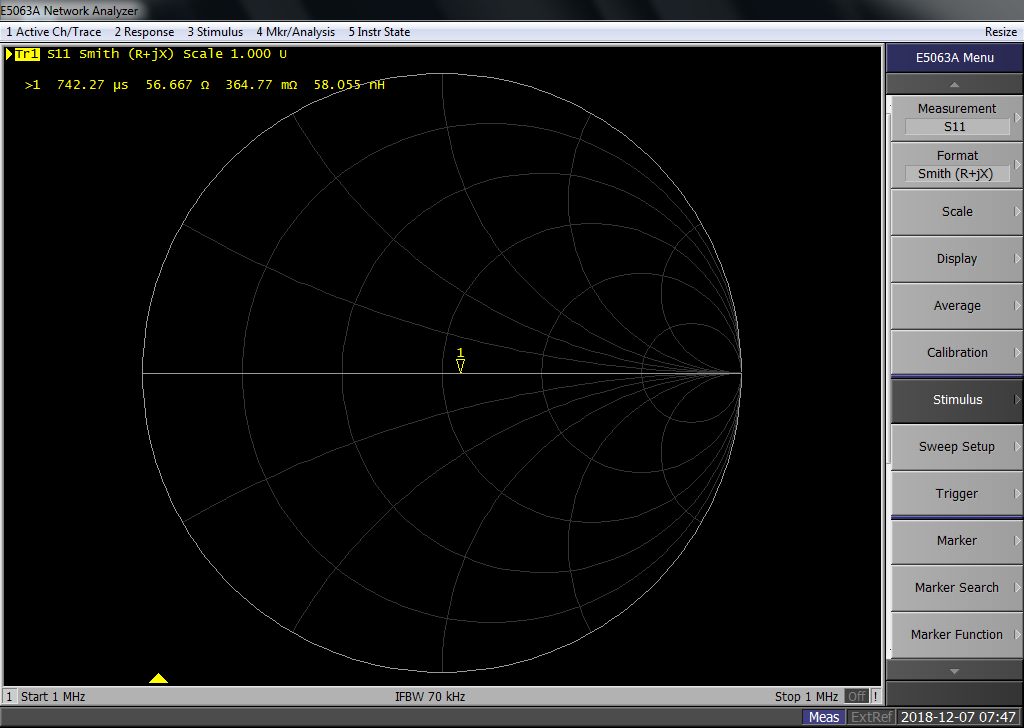
\includegraphics[width=2.5in]{./img/smith_50_ohms_1_MHz.png}
  \caption{Smith Chart: \SI{50}{\ohm} Resistor, 1 MHz}
  \label{fig:smith_50_ohms_1_MHz}
\end{figure}

\begin{figure}[H]
  \centering
  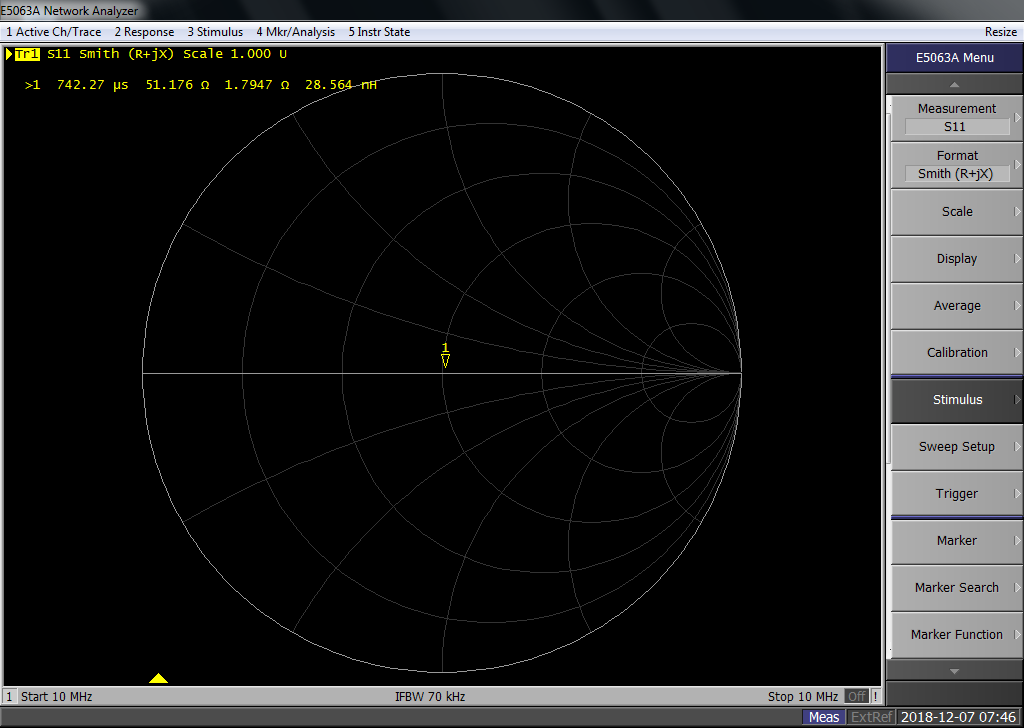
\includegraphics[width=2.5in]{./img/smith_50_ohms_10_MHz.png}
  \caption{Smith Chart: \SI{50}{\ohm} Resistor, 10 MHz}
  \label{fig:smith_50_ohms_10_MHz}
\end{figure}

\begin{figure}[H]
  \centering
  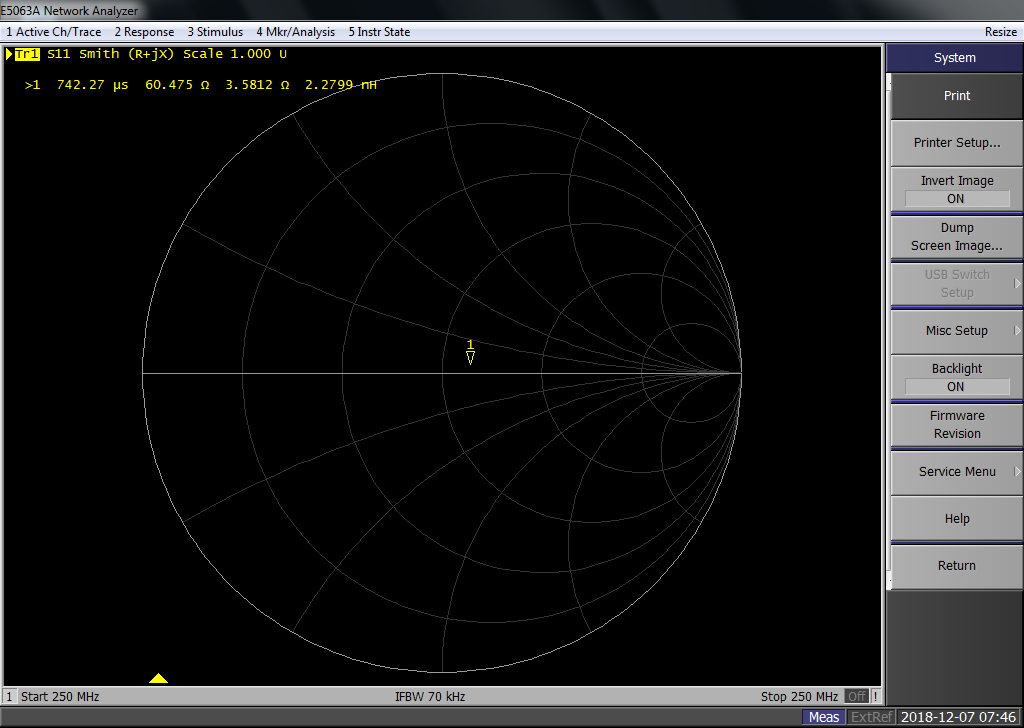
\includegraphics[width=2.5in]{./img/smith_50_ohms_250_MHz.png}
  \caption{Smith Chart: \SI{50}{\ohm} Resistor, 250 MHz}
  \label{fig:smith_50_ohms_250_MHz}
\end{figure}

\begin{figure}[H]
  \centering
  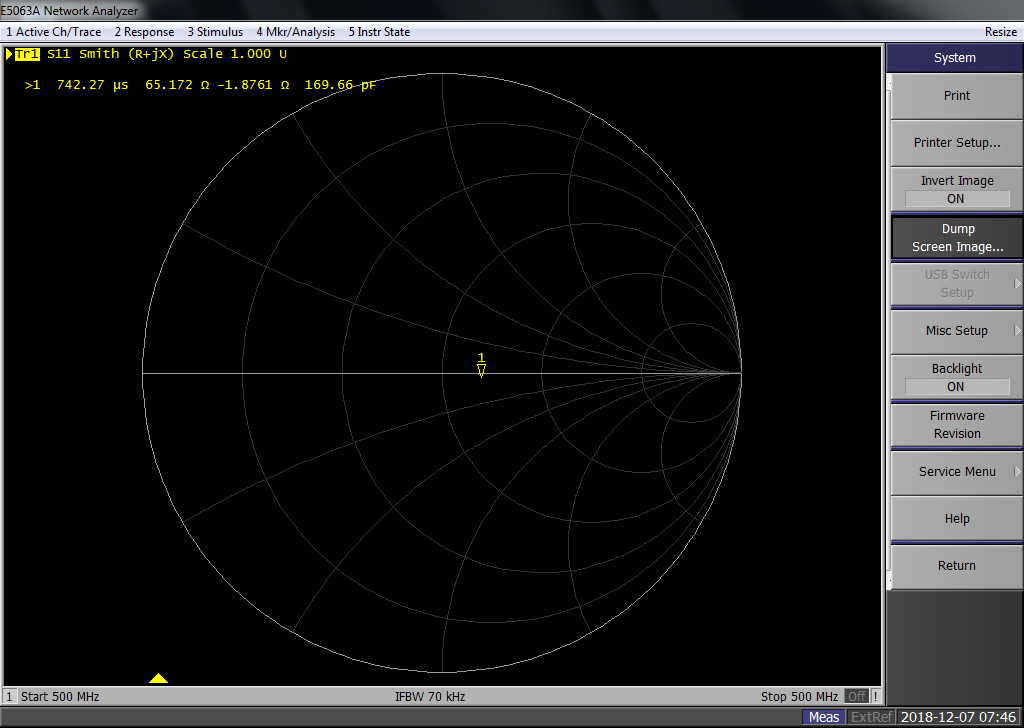
\includegraphics[width=2.5in]{./img/smith_50_ohms_500_MHz.png}
  \caption{Smith Chart: \SI{50}{\ohm} Resistor, 500 MHz}
  \label{fig:smith_50_ohms_500_MHz}
\end{figure}

\subsection{\SI{100}{\ohm} Resistor}

\begin{figure}[H]
  \centering
  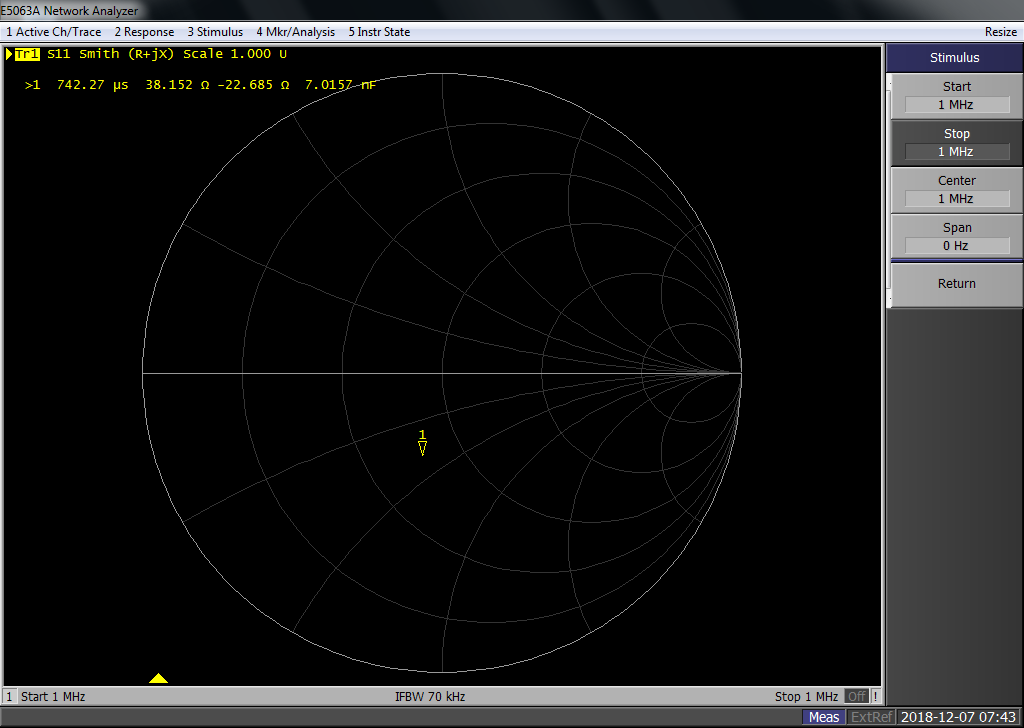
\includegraphics[width=2.5in]{./img/smith_100_ohms_1_MHz.png}
  \caption{Smith Chart: \SI{100}{\ohm} Resistor, 1 MHz}
  \label{fig:smith_100_ohms_1_MHz}
\end{figure}

\begin{figure}[H]
  \centering
  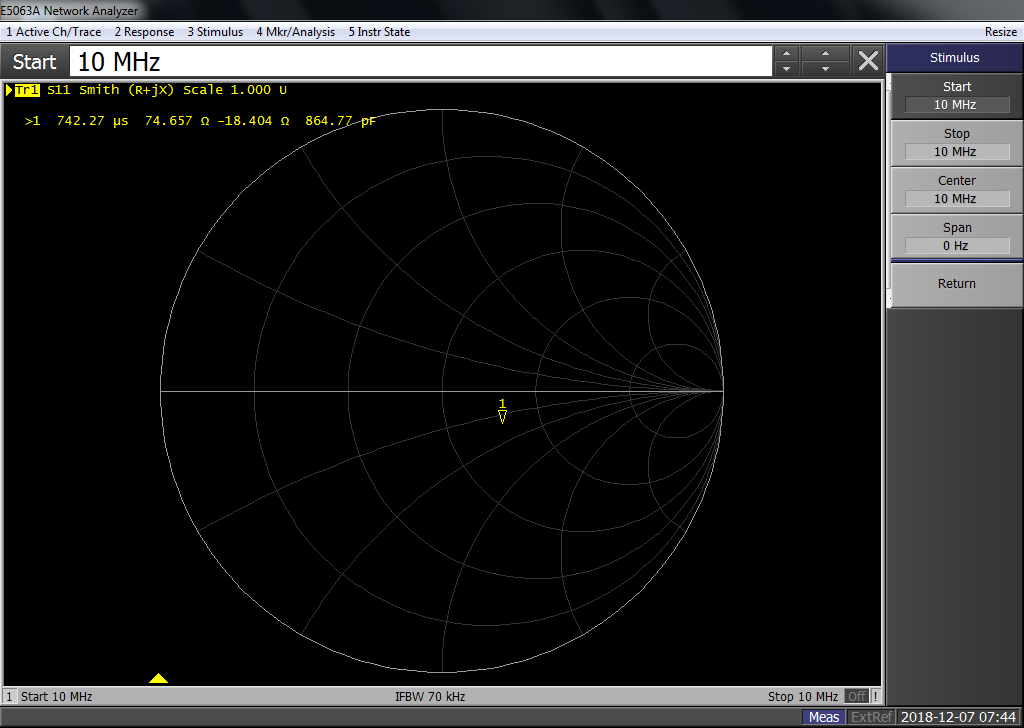
\includegraphics[width=2.5in]{./img/smith_100_ohms_10_MHz.png}
  \caption{Smith Chart: \SI{100}{\ohm} Resistor, 10 MHz}
  \label{fig:smith_100_ohms_10_MHz}
\end{figure}

\begin{figure}[H]
  \centering
  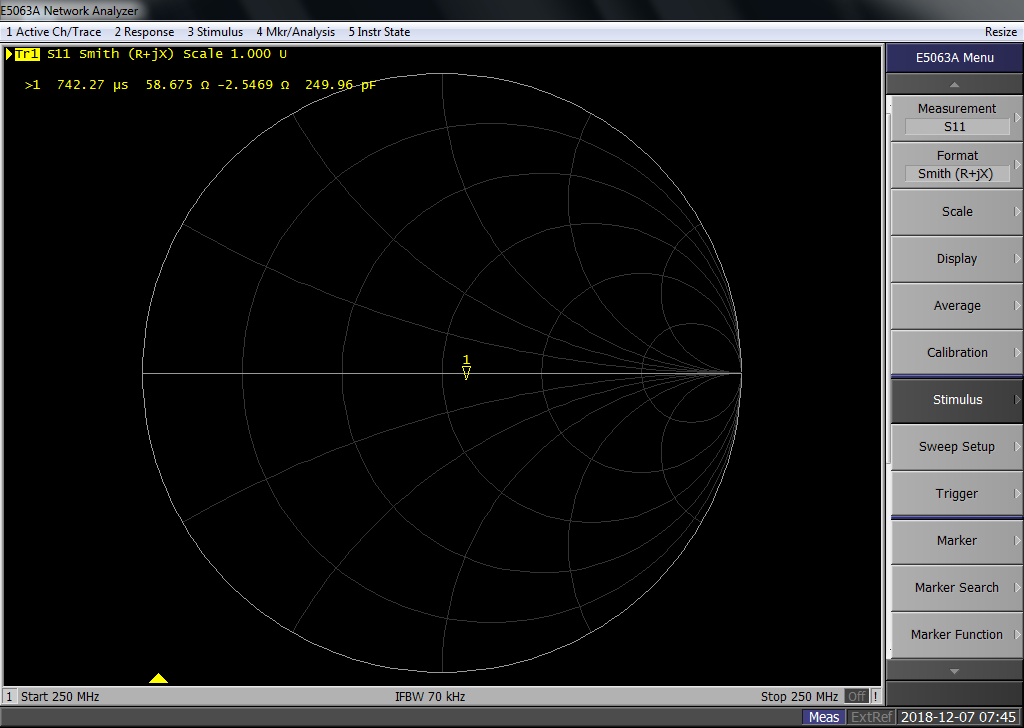
\includegraphics[width=2.5in]{./img/smith_100_ohms_250_MHz.png}
  \caption{Smith Chart: \SI{100}{\ohm} Resistor, 250 MHz}
  \label{fig:smith_100_ohms_250_MHz}
\end{figure}

\begin{figure}[H]
  \centering
  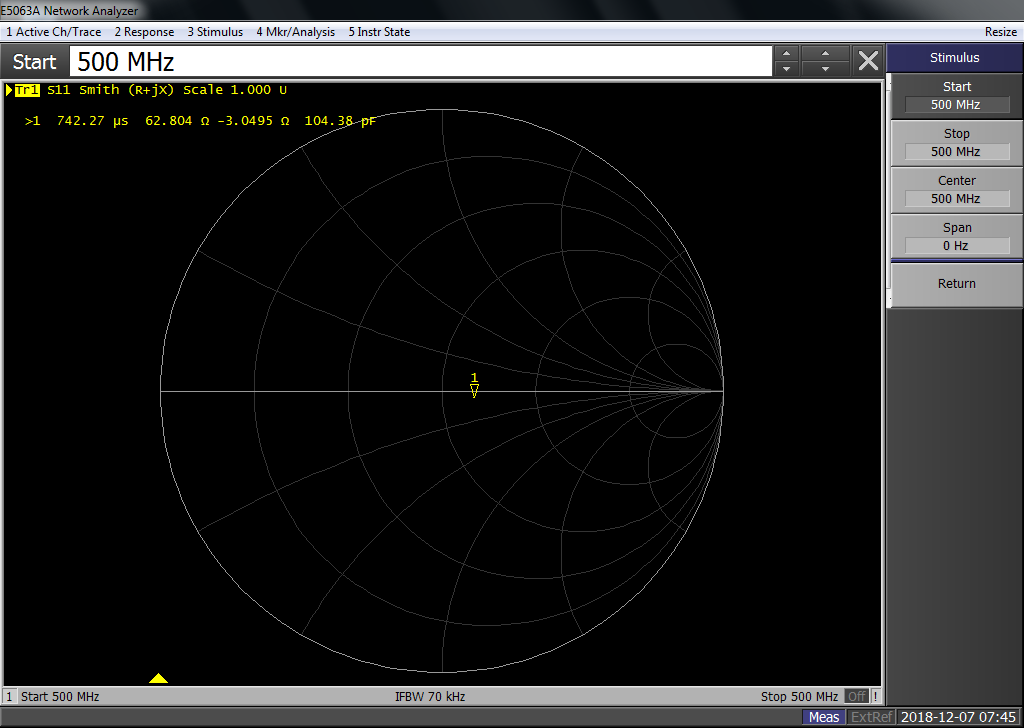
\includegraphics[width=2.29in]{./img/smith_100_ohms_500_MHz.png}
  \caption{Smith Chart: \SI{100}{\ohm} Resistor, 500 MHz}
  \label{fig:smith_100_ohms_500_MHz}
\end{figure}

\subsection{\SI{2.2}{\pico\farad} Capacitor}

\begin{figure}[H]
  \centering
  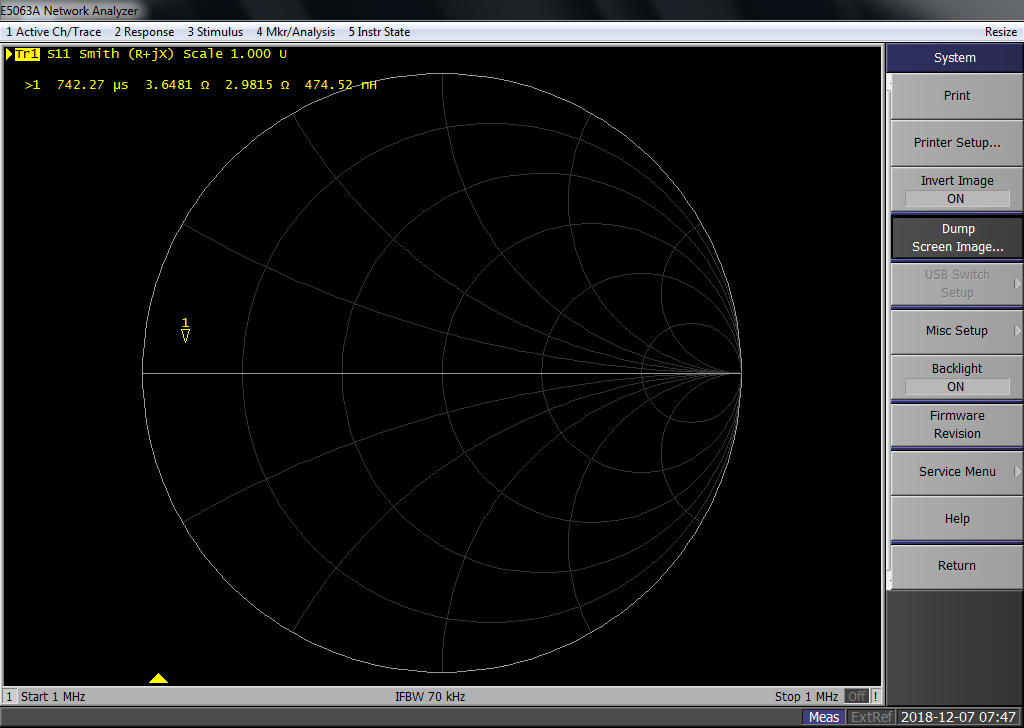
\includegraphics[width=2.5in]{./img/smith_2_pF_1_MHz.png}
  \caption{Smith Chart: \SI{2.2}{\pico\farad} Capacitor, 1 MHz}
  \label{fig:smith_2_pF_1_MHz}
\end{figure}

\begin{figure}[H]
  \centering
  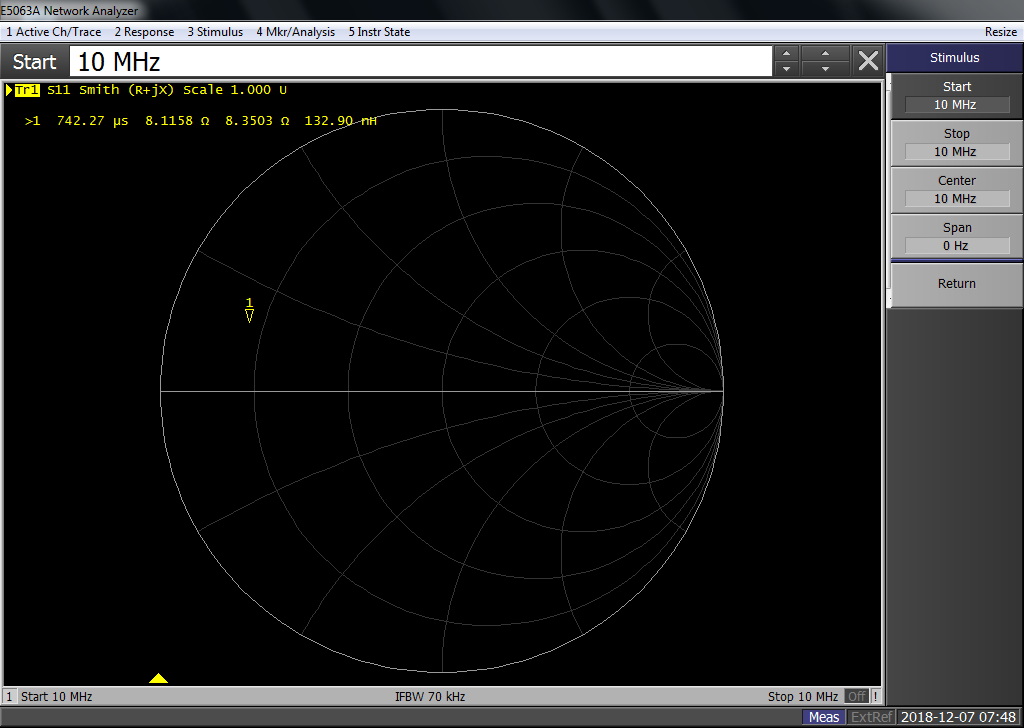
\includegraphics[width=2.5in]{./img/smith_2_pF_10_MHz.png}
  \caption{Smith Chart: \SI{2.2}{\pico\farad} Capacitor, 10 MHz}
  \label{fig:smith_2_pF_10_MHz}
\end{figure}

\begin{figure}[H]
  \centering
  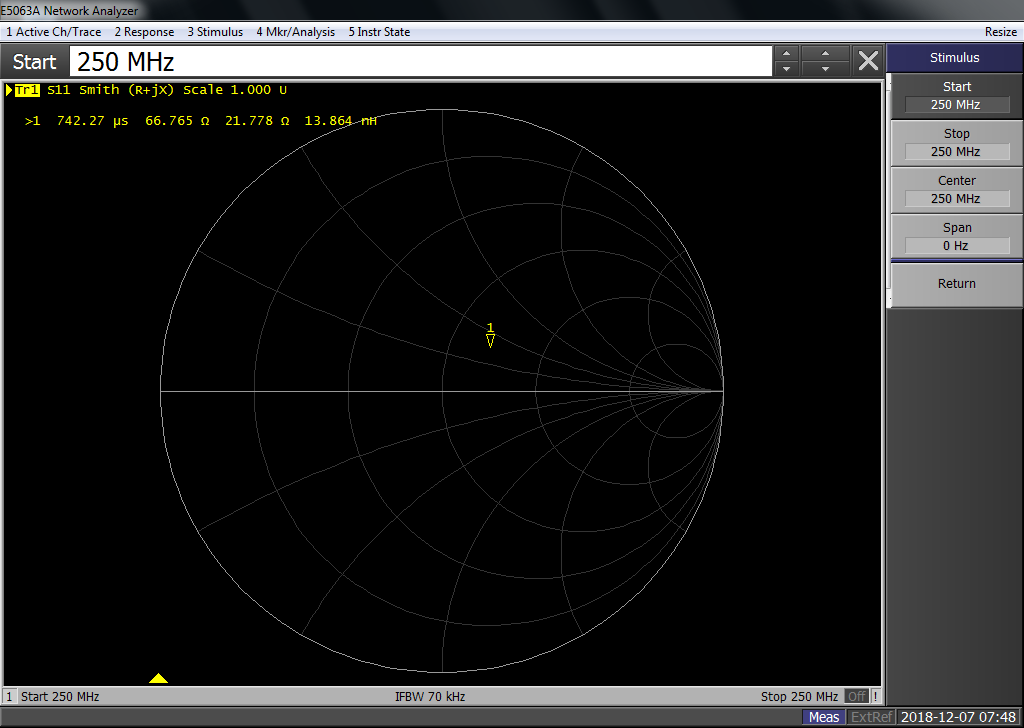
\includegraphics[width=2.5in]{./img/smith_2_pF_250_MHz.png}
  \caption{Smith Chart: \SI{2.2}{\pico\farad} Capacitor, 250 MHz}
  \label{fig:smith_2_pF_250_MHz}
\end{figure}

\begin{figure}[H]
  \centering
  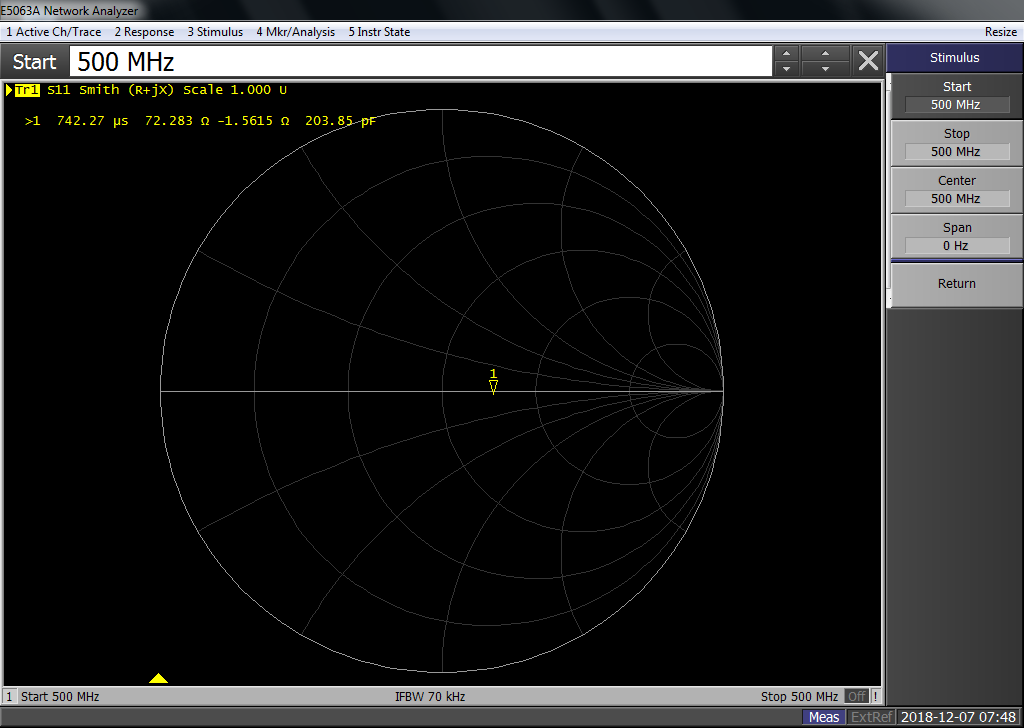
\includegraphics[width=2.29in]{./img/smith_2_pF_500_MHz.png}
  \caption{Smith Chart: \SI{2.2}{\pico\farad} Capacitor, 500 MHz}
  \label{fig:smith_2_pF_500_MHz}
\end{figure}

\subsection{Short Circuit}

\begin{figure}[H]
  \centering
  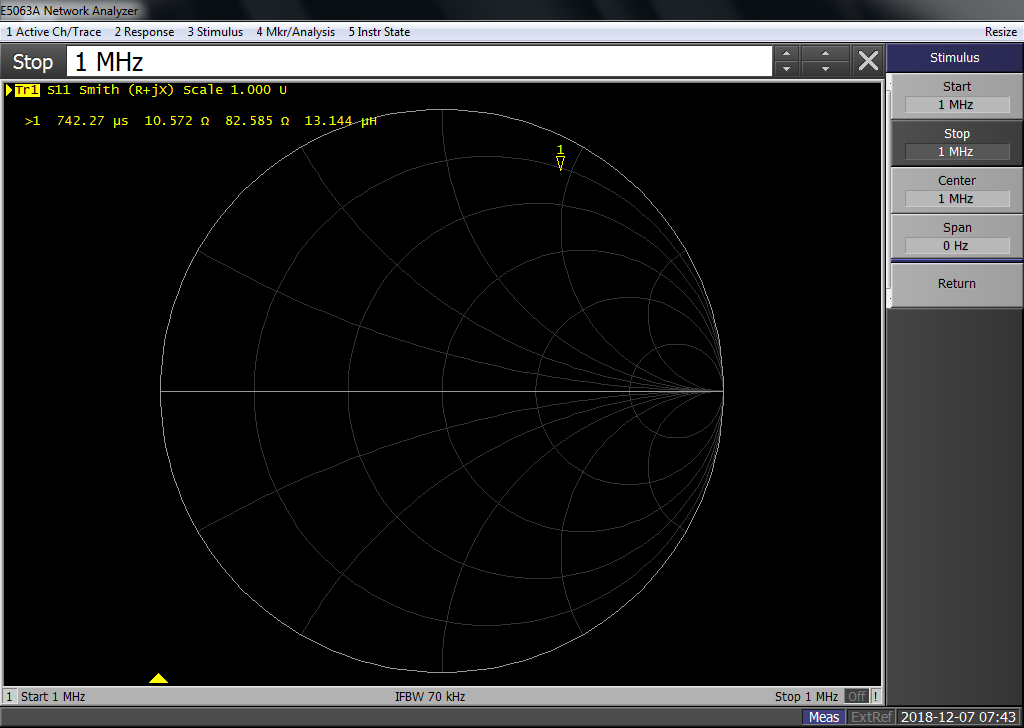
\includegraphics[width=2.5in]{./img/smith_short_1_MHz.png}
  \caption{Smith Chart: Short Circuit, 1 MHz}
  \label{fig:smith_short_1_MHz}
\end{figure}

\begin{figure}[H]
  \centering
  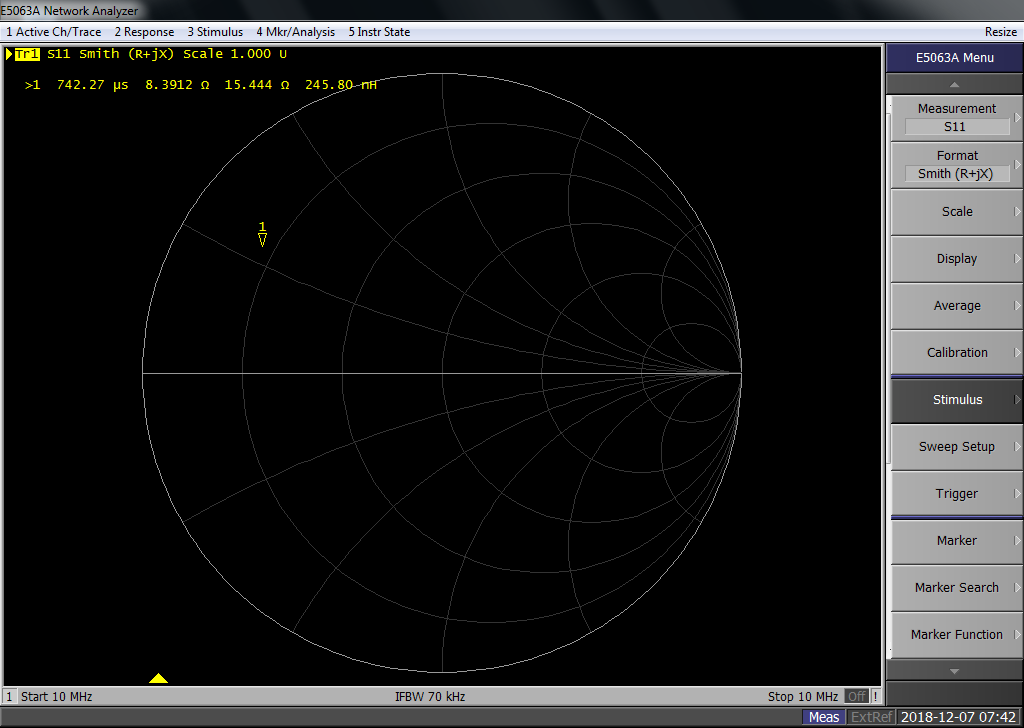
\includegraphics[width=2.5in]{./img/smith_short_10_MHz.png}
  \caption{Smith Chart: Short Circuit, 10 MHz}
  \label{fig:smith_short_10_MHz}
\end{figure}

\begin{figure}[H]
  \centering
  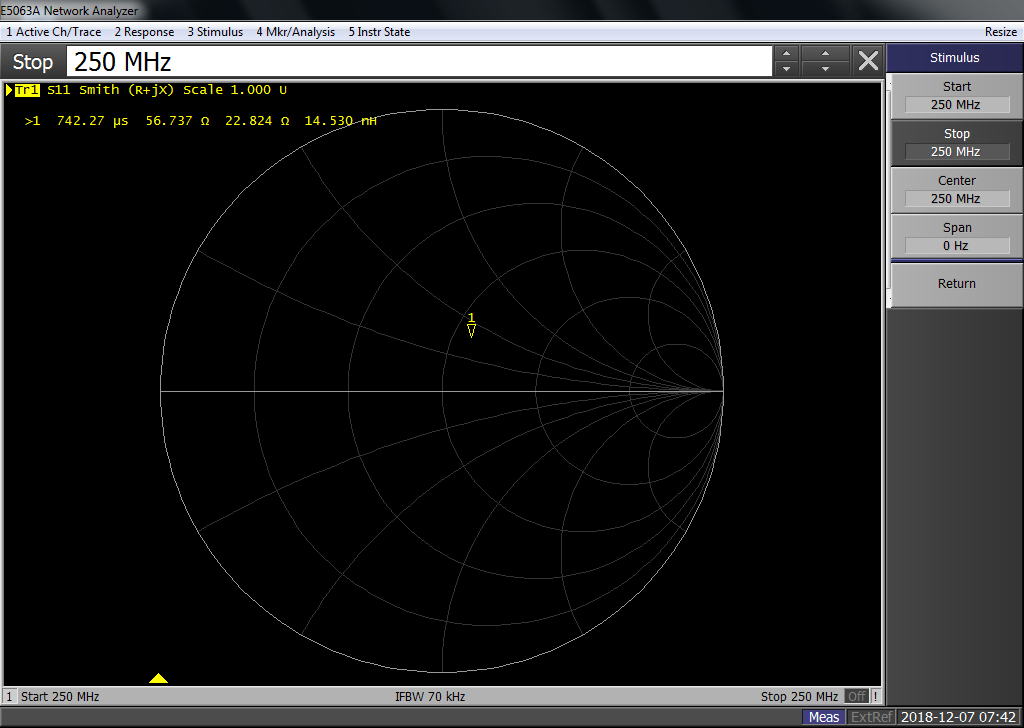
\includegraphics[width=2.5in]{./img/smith_short_250_MHz.png}
  \caption{Smith Chart: Short Circuit, 250 MHz}
  \label{fig:smith_short_250_MHz}
\end{figure}

\begin{figure}[H]
  \centering
  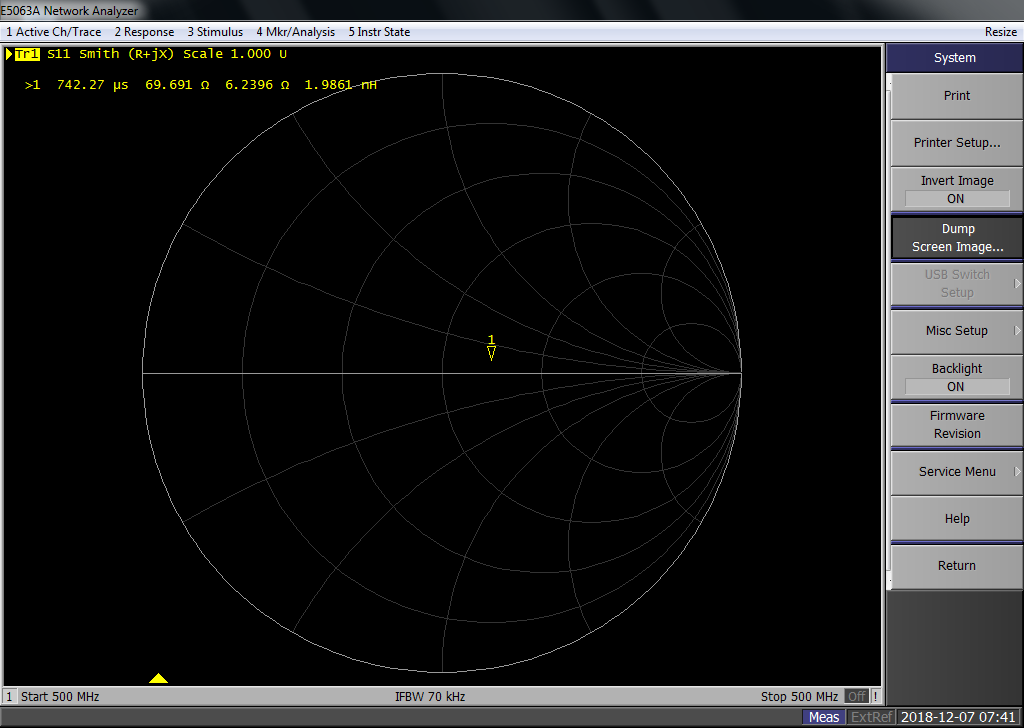
\includegraphics[width=2.29in]{./img/smith_short_500_MHz.png}
  \caption{Smith Chart: Short Circuit, 500 MHz}
  \label{fig:smith_short_500_MHz}
\end{figure}

\subsection{Open Circuit}

\begin{figure}[H]
  \centering
  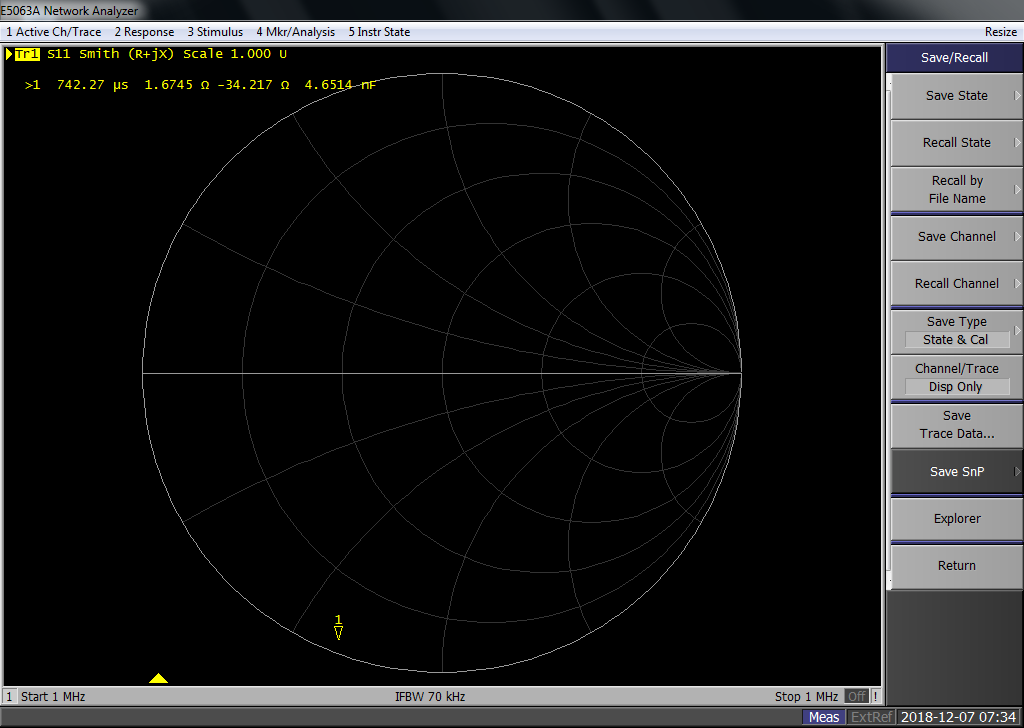
\includegraphics[width=2.5in]{./img/smith_open_1_MHz.png}
  \caption{Smith Chart: Open Circuit, 1 MHz}
  \label{fig:smith_open_1_MHz}
\end{figure}

\begin{figure}[H]
  \centering
  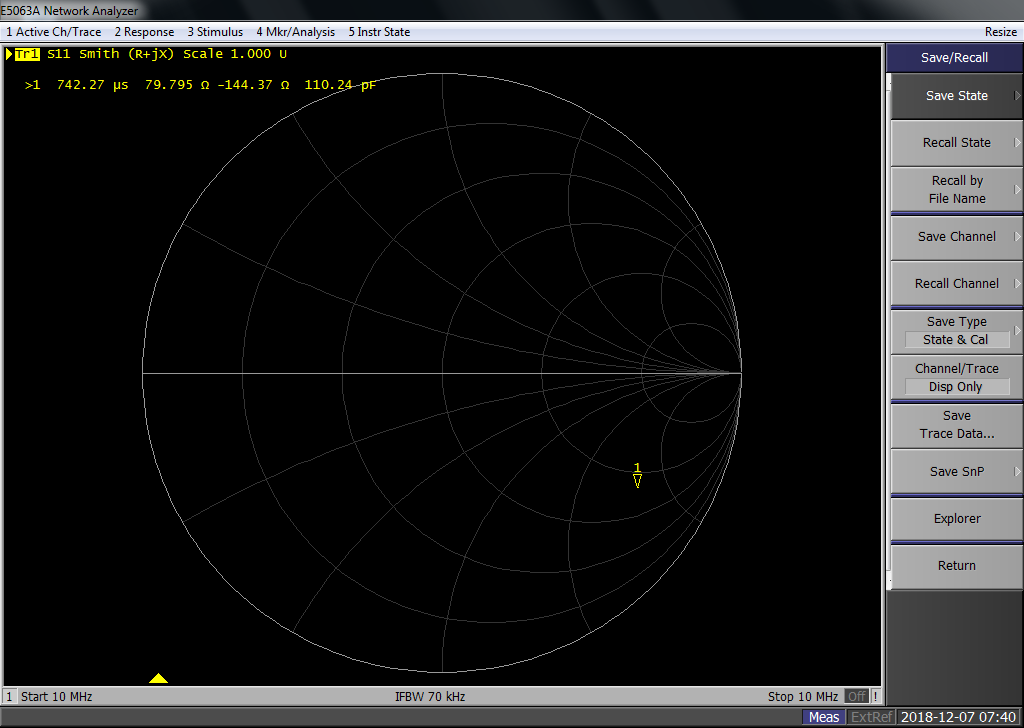
\includegraphics[width=2.5in]{./img/smith_open_10_MHz.png}
  \caption{Smith Chart: Open Circuit, 10 MHz}
  \label{fig:smith_open_10_MHz}
\end{figure}

\begin{figure}[H]
  \centering
  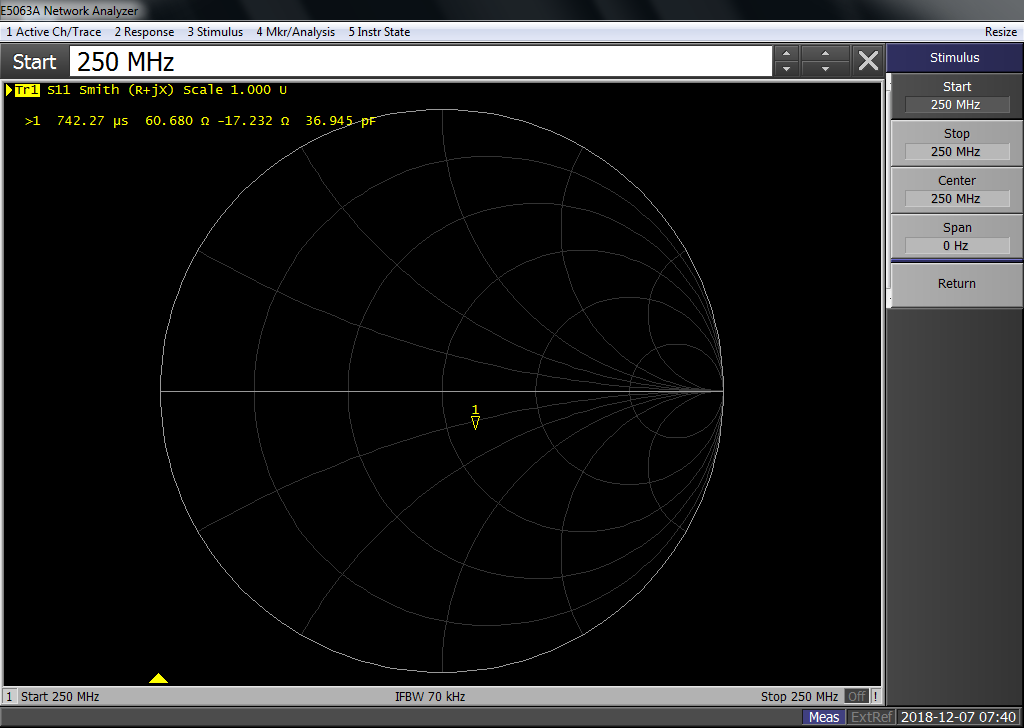
\includegraphics[width=2.5in]{./img/smith_open_250_MHz.png}
  \caption{Smith Chart: Open Circuit, 250 MHz}
  \label{fig:smith_open_250_MHz}
\end{figure}

\begin{figure}[H]
  \centering
  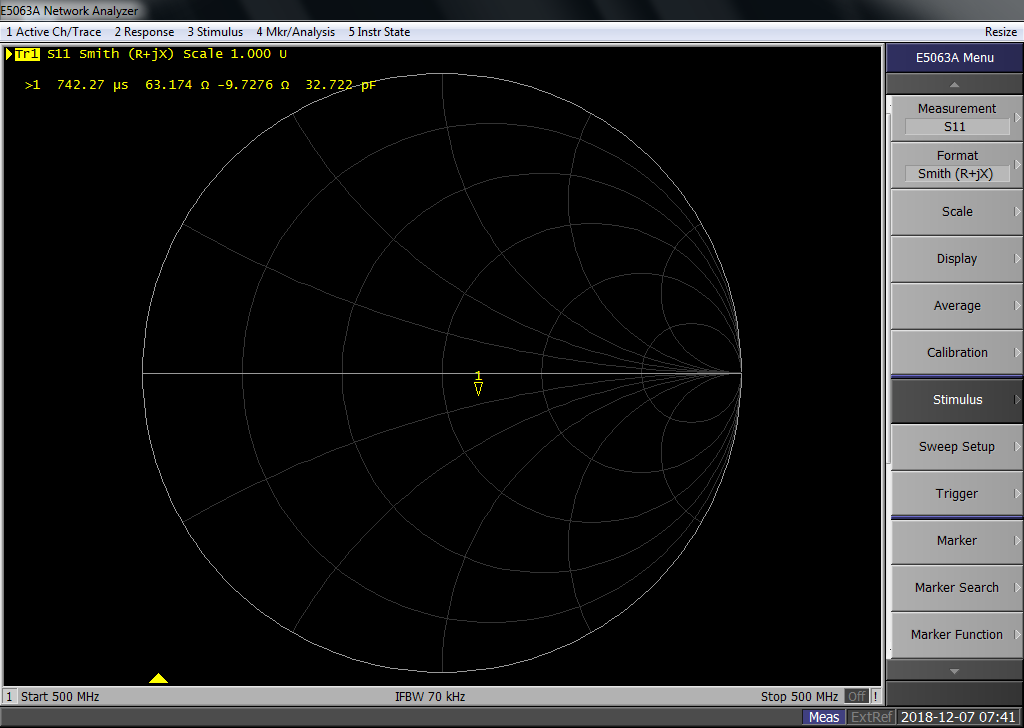
\includegraphics[width=2.29in]{./img/smith_open_500_MHz.png}
  \caption{Smith Chart: Open Circuit, 500 MHz}
  \label{fig:smith_open_500_MHz}
\end{figure}

\section{$Z_0$ Calculations}
Using Equation \ref{eq:z_0}, Equation \ref{eq:z_in} and the network analyzer values for the input
impedance of the open and short circuits for the transmission line, it is
possible to calculate $Z_0$ and $\gamma$.
\[
  \begin{array}{ll}
    \gamma = \frac{\arctanh{(\frac{Z_0 (Z_{in}-Z_L)}{Z_0^2-Z_{in} Z_L})} +
      j\pi n}{l}\\
    n \in \mathbb{Z}\\
  \end{array}
  \]

\subsection{1 MHz}
\begin{equation}{\label{eq:z_0_1_MHz}}
  \begin{array}{ll}
    Z_{in}^{OC} = 10.574 + j82.585\\
    Z_{in}^{SC} = 1.6745 - j34.217\\
    Z_0 = \sqrt{(10.574 + j82.585)(1.6745 - j34.217)}\\
    Z_0 = 53.4068 - j2.09\\
    \gamma = \num{1.33e-3} + j\num{2.952e-1}
  \end{array}
\end{equation}
(Figures \ref{fig:smith_short_1_MHz} and \ref{fig:smith_open_1_MHz})
)
\subsection{10 MHz}
\begin{equation}{\label{eq:z_0_10_MHz}}
  \begin{array}{ll}
    Z_{in}^{OC} = 8.3912 + j15.444\\
    Z_{in}^{SC} = 79.795 - j144.37\\
    Z_0 = \sqrt{(8.3912 + j15.444)(79.795.37 - 144.37)}\\
    Z_0 = 53.8452 + j0.1942\\
    \gamma = \num{4.86e-3} + j \num{2.713e-1}
  \end{array}
\end{equation}
(Figures \ref{fig:smith_short_10_MHz} and \ref{fig:smith_open_10_MHz})

\subsection{250 MHz}
\begin{equation}{\label{eq:z_0_250_MHz}}
  \begin{array}{ll}
    Z_{in}^{OC} = 56.737 + j22.8524\\
    Z_{in}^{SC} = 60.680 - j17.232\\
    Z_0 = \sqrt{(56.737 + j22.8524)(60.680 - j17.232)}\\
    Z_0 = 62.12 + j3.30\\
    \gamma = \num{4.86e-3} + j\num{2.713e-1}
  \end{array}
\end{equation}
(Figures \ref{fig:smith_short_250_MHz} and \ref{fig:smith_open_250_MHz})

\subsection{500 MHz}
\begin{equation}{\label{eq:z_0_500_MHz}}
  \begin{array}{ll}
    Z_{in}^{OC} = 69.691 + j6.2396\\
    Z_{in}^{SC} = 63.174 - j9.7276\\
    Z_0 = \sqrt{(69.691 + j6.2396)(63.174 - j9.7276)}\\
    Z_0 = 66.84 - j2.12\\
    \gamma = \num{4.86e-3} + j \num{2.713e-1}
  \end{array}
\end{equation}

(Figures \ref{fig:smith_short_500_MHz} and \ref{fig:smith_open_500_MHz})

\section{$Z_L$ Calculations}
Using the theoretical $Z_0$ and $\gamma$ values, as well as the measured
$Z_{in}$, a theoretical $Z_L$ can be
calculated using Equation \ref{eq:z_in} for each transmission line.

\[
  \begin{array}{ll}
    Z_L = \frac{-(e^{2\gamma l} (Z_0-Z_{in})Z0}{e^{2\gamma l}
      (Z_0-Z_{in})+Z_0+Z_{in}}
  \end{array}
\]

\subsection{\SI{50}{\ohm} Resistor}
Sample Calculation, \SI{50}{\ohm} at 1 MHz (Figure
\ref{fig:smith_50_ohms_1_MHz}).

\[
  \begin{array}{ll}
  \Scale[0.5]{
    Z_L = \frac{-(e^{2(\num{4.86e-3} + j \num{2.713e-1})(30)} ((53.4068 -
      j2.09)-(56.67 + j364.77)) (53.4068 -
      j2.09)}{e^{2(\num{4.86e-3} + j \num{2.713e-1})(30)}
      ((53.4068 -
      j2.09)-(56.67 + j364.77))+(53.4068 -
      j2.09)+(56.67 + j364.77)}
  }\\
  Z_L = -9.215 -j2.355
  \end{array}
  \]

  \SI{50}{\ohm} at 10 MHz (Figure \ref{fig:smith_50_ohms_10_MHz}).

  \[
    \begin{array}{ll}
      Z_L = -9.215 - j2.355
    \end{array}
  \]

  \SI{50}{\ohm} at 250 MHz (Figure \ref{fig:smith_50_ohms_250_MHz}).

  \[
    \begin{array}{ll}
      Z_L = -9.215 - j2.355
    \end{array}
  \]

  \SI{50}{\ohm} at 500 MHz (Figure \ref{fig:smith_50_ohms_500_MHz}).

  \[
    \begin{array}{ll}
      Z_L = -9.215 - j2.355
    \end{array}
  \]

\subsection{\SI{100}{\ohm} Resistor}
\SI{100}{\ohm} at 1 MHz (Figure
\ref{fig:smith_100_ohms_1_MHz}).

\[
  \begin{array}{ll}
    Z_L = 37.2 + j 48.9
  \end{array}
  \]

  \SI{100}{\ohm} at 10 MHz (Figure \ref{fig:smith_100_ohms_10_MHz}).

  \[
    \begin{array}{ll}
      Z_L = 37.2 + j48.9
    \end{array}
  \]

  \SI{100}{\ohm} at 250 MHz (Figure \ref{fig:smith_100_ohms_250_MHz}).

  \[
    \begin{array}{ll}
      Z_L = 58.8 - j2.55
    \end{array}
  \]

  \SI{100}{\ohm} at 500 MHz (Figure \ref{fig:smith_100_ohms_500_MHz}).

  \[
    \begin{array}{ll}
      Z_L = 62.8 - j3.05
    \end{array}
  \]


\subsection{\SI{2}{\farad} Capacitor}
\SI{2}{\pico\farad} at 1 MHz (Figure
\ref{fig:smith_2_pF_1_MHz}).

\[
  \begin{array}{ll}
    Z_L = 3.65 + j2.98\\
    %Z_L = \frac{1}{j \omega C_L}
    %C_L = \frac{1}{j \omega Z_L}
    %C_L = \frac{1}{(1M) j(3.65 + j2.98)}
    %C_L = 
  \end{array}
  \]

  \SI{2}{\pico\farad} at 10 MHz (Figure \ref{fig:smith_2_pF_10_MHz}).

  \[
    \begin{array}{ll}
      Z_L = 37.2 + j48.9
    \end{array}
  \]

  \SI{2}{\pico\farad} at 250 MHz (Figure \ref{fig:smith_2_pF_250_MHz}).

  \[
    \begin{array}{ll}
      Z_L = 66.765 + j2.18
    \end{array}
  \]

  \SI{2}{\pico\farad} at 500 MHz (Figure \ref{fig:smith_2_pF_500_MHz}).

  \[
    \begin{array}{ll}
      Z_L = 72.283 -j1.56
    \end{array}
  \]

\end{document}
